\subsection{Motivations}
\begin{frame}{Background}

\begin{itemize}
    \item A preliminary study on RKB for collaborative learning has explained how the approach affects collaborative learning outcomes and students’ learning experiences[12]; however, it does not investigate how individual prior knowledge convergence and comprehension levels through reconstruction may potentially influence the final collaborative product.
    \item It also does not identify how knowledge is potentially transferred from individual solutions, according to the similarity of knowledge and comprehension levels between the group members. Thus, the current study aims to address those issues.
    \item Identifying the relationship between the individual and group product is important since there is interdependence between these two. The results of this study highlight the role of individual phases of RKB activities in foreseeing students’ learning achievements as a group.
\end{itemize}
       
\end{frame}

\begin{frame}{Sub-research questions}

\textcolor<1>{blue}{Aim}: To identify which phase is important during RKB

\begin{block}{RQs}
    \begin{enumerate}
        %\setcounter{enumii}{1}
        \item Does similarity of individual prior knowledge and/or comprehension 
              of partner's representation predict group learning outcomes?
        \item How similarity of individual prior knowledge and comprehension
              of partner's representation contribute to group learning outcomes?
    \end{enumerate}
\end{block}
    
\end{frame}



\subsection{Analysis methods}
\begin{frame}[allowframebreaks]{Data measurements (1): Similarity of prior knowledge}
    \begin{enumerate}
        \item A graph \textit{G} = (\textit{V}, \textit{E}) is a finite set $V$ 
        of $n$ nodes and a set \textit{E} of edges, where \textit{E} is a 
        subset of $V \times V$.
        \item Given two undirected and labeled graphs, $A = (V, E_A)$ and 
        $B = (V, E_B)$, with common node set $V$, $S(A, B)$ is the similarity 
        between $A$ and $B$ as measured by $S$. 
        \item $SE_{AB}$ consists of shared links between $E_A$ and $E_B$ 
        while $UE_{AB}$ contains a set of unshared links created by 
        only one of the group members.
    \end{enumerate}
     
    \begin{equation}
      SE_{AB} = E_A \cap E_B \label{eq:1}
    \end{equation}
    
    \begin{equation}
      UE_{AB} = E_A \ominus E_B \label{eq:2}
    \end{equation}
    
    \begin{equation}
      S(A, B) = \frac{|SE_{AB}|}{{|SE_{AB}| + \frac{|UE_{AB}|}{2}}} \label{eq:3}
    \end{equation}
    
    \begin{itemize}
        \item Linking words similarity
        \item Term Frequency - Inverse Document Frequency (TF-IDF) cosine similarity
              formula 
        \item Pre-processing techniques: text normalization 
              (e.g., transforming to lower case, removing punctuation, stemming) 
              and stop-word removal
        \item Linking-word similarity falls into three following categories: 
        \begin{itemize}
            \item \textbf{no similarity} if the score is 0; 
            \item \textbf{moderately low similarity} if the score lies between 0--.509;
            \item \textbf{moderately high similarity} if greater than .509.
        \end{itemize} 
        \item This categorization is based on the first and third quartiles 
        of the similarity score distribution ($M = .27, SD = .34, Q1 = 0, Q3 = .509$).
    \end{itemize}


\end{frame}

\begin{frame}[allowframebreaks]{Data measurements (2): Comprehension of partner's map components}
    
    
    \begin{itemize}
        \item The element of $E_{MA}$ is called a reconstructed link, while $E_{NA}$
              consists of non-reconstructed links.
                \begin{equation}
                    E_{MA} = E_{RA} \cap E_A 
                \end{equation}
                \begin{equation}
                    E_{NA} = E_{RA} \ominus E_A
                \end{equation}
        \item Given two undirected and labeled re-constructional graphs $R_A$ and 
              $R_B$ with common node set $V$, 
              $C(A, B)$ is the comprehension value between student 
              $A$ and $B$, as a pair in a group, defined as:
              \begin{equation}
                C(A, B) = \frac{|E_{MA} + E_{MB}|}{|E_{MA} + E_{MB}| + \frac{|E_{NA} + E_{NB}|}{2}} 
              \label{eq:6}
            \end{equation}
    \end{itemize}
    
    
By applying the TF-IDF cosine similarity formula \cite{Qian2004SimilarityQueries}
and some pre-processing techniques, the similarity score is calculated.
The similarity value is from 0 to 1 inclusive, with
the mean of .68 and standard deviation of .37. 
Furthermore, the first and third quartiles  
of the data distribution are used to define thresholds for categorization
($Q1 = .366, Q3 = 1$). The categories of individual-to-group linking word 
similarity are as follows:
\begin{itemize}
\item \textbf{follow initial}: the group of linking words that are similar with 
at least one of the individual linking words (similarity value of equal to or more than .99);
\item \textbf{modify initial}: the group of linking words that are modified from one 
of the individual linking words (similarity value above .366 and below .99);
\item \textbf{new}: the group of linking words that are 
not similar to any of the individual linking words 
(similarity value of below .366).
\end{itemize}


\end{frame}

\begin{frame}{Data measurements (3): Map Score Change}

To measure the change of map score from the individual to the collaborative phase, this 
study adopts the normalized change formula proposed by Marx and Cummings 

%\cite{Marx2007NormalizedChange}.

\begin{equation}
 c =
    \begin{cases}
        \frac{gms - ais}{100 - ais} & \text{if $gms$ > $ais$}\\
        $drop$ & \text{if $gms$ = $ais$ = 100 or 0} \\
        0 & \text{if $gms$ = $ais$}\\
        \frac{gms - ais}{ais} & \text{if $gms$ < $ais$}
    \end{cases}
    \label{eq:7}
\end{equation}
    
\end{frame}


\subsection{Results \& discussions}
\begin{frame}{Results (1): Relationship Between Group Prior Knowledge Similarity, 
   Comprehension of the Partner’s Kit, and Map Score Change}

\begin{table}[tb]
    \caption{Descriptive statistics}
    \label{desc_stat}
    \begin{center}
        \begin{tabular}{c|c|c|c|c}
            \hline
            Data & $M$ & $SD$ & $Min$ & $Max$\\
            \hline
            $S(A, B)$ & .47 & .27 & 0 & .93 \\
            $C(A, B)$ & .85 & .12 & .65 & 1 \\
            & & & &\\
            $ais$ & 72.21 & 18.22 & 41.43 & 98.57 \\
            $gms$ & 90 & 7.31 & 75.71 & 100 \\
            $c$ & .54 & .34 & -.09 & 1 \\
            \hline
        \end{tabular}
    \end{center}
\end{table}
\end{frame}


\begin{frame}{Results (1): Relationship Between Group Prior Knowledge Similarity, 
   Comprehension of the Partner’s Kit, and Map Score Change}
    \begin{columns}
        \begin{column}{0.5\textwidth}
            \begin{center}
                \begin{figure}[tb]
                    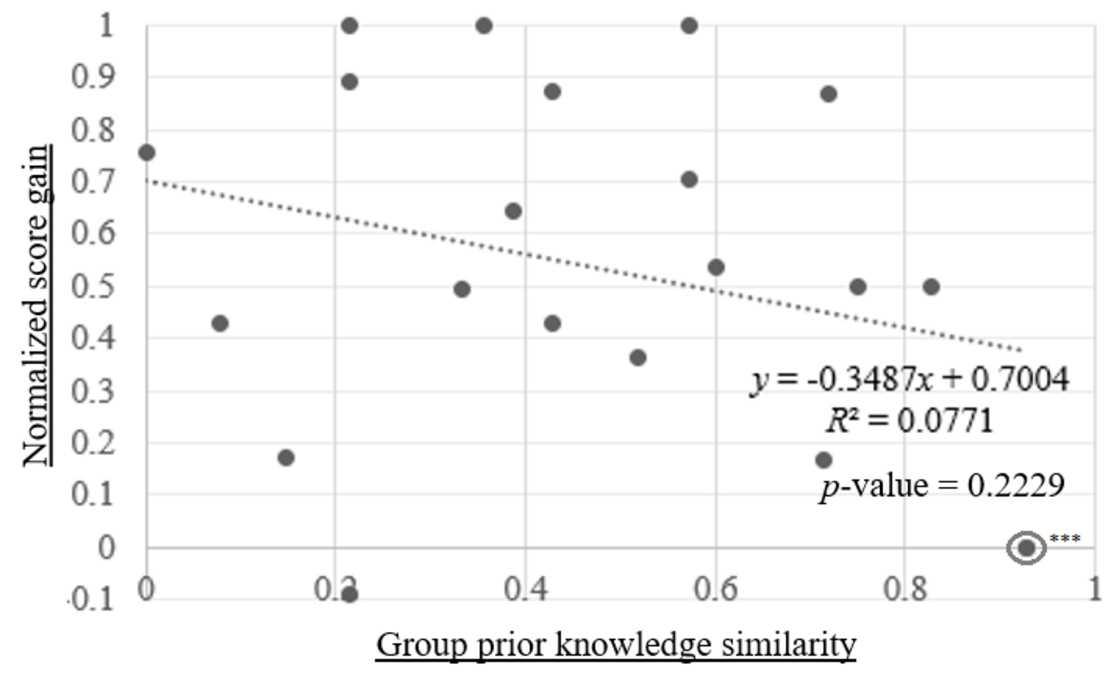
\includegraphics[width=60mm]{/images/a3_prior_gain_plot.pdf}
                    \caption{Scatter plot of group prior knowledge similarity and normalized gain from individual to collaborative map}
                    \label{prior_gain}
                \end{figure}
            \end{center}
        \end{column}
        \begin{column}{0.5\textwidth}  %%<--- here
            \begin{center}
                \begin{figure}[tb]
                    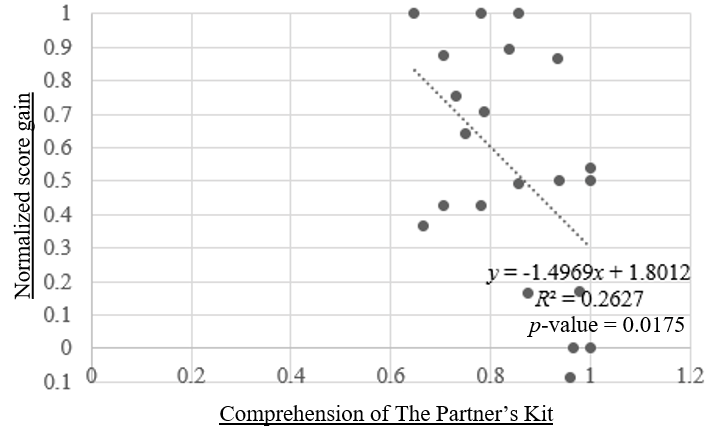
\includegraphics[width=60mm]{/images/a3_comprehension_gain_plot.pdf}
                    \caption{Scatter plot of group comprehension level and normalized gain from 
                    individual to collaborative map}
                    \label{comprehension_gain}
                \end{figure}
            \end{center}
        \end{column}
    \end{columns} 
\end{frame}

\begin{frame}{Results (1): Relationship Between Group Prior Knowledge Similarity, 
   Comprehension of the Partner’s Kit, and Map Score Change}
\begin{figure}[tb]
    \begin{center}
        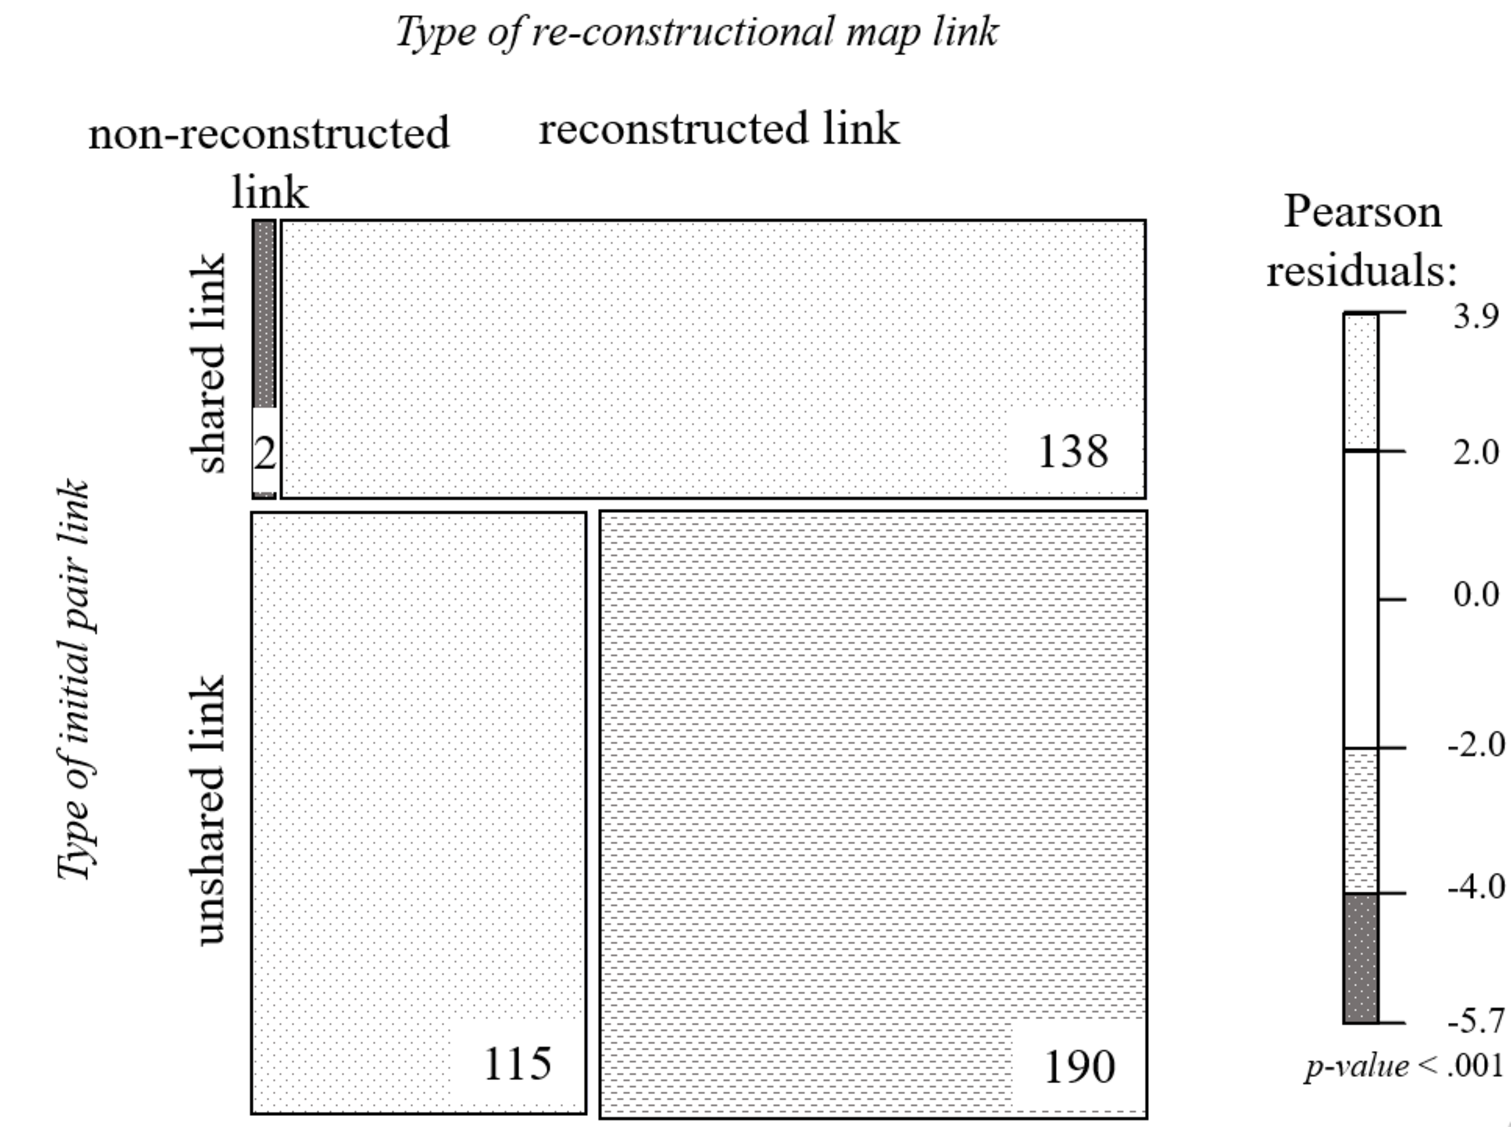
\includegraphics[width=70mm]{images/a3_prior_comprehension_distribution.pdf}
    \end{center}
    \caption{Mosaic plot of similarity of prior knowledge and comprehension of partner's kit}
    \label{prior_comprehension_dist}
\end{figure}
\end{frame}

\begin{frame}{Results (2): Individual Contributions to Collaborative Products}
    \begin{figure}[tb]
        \begin{center}
            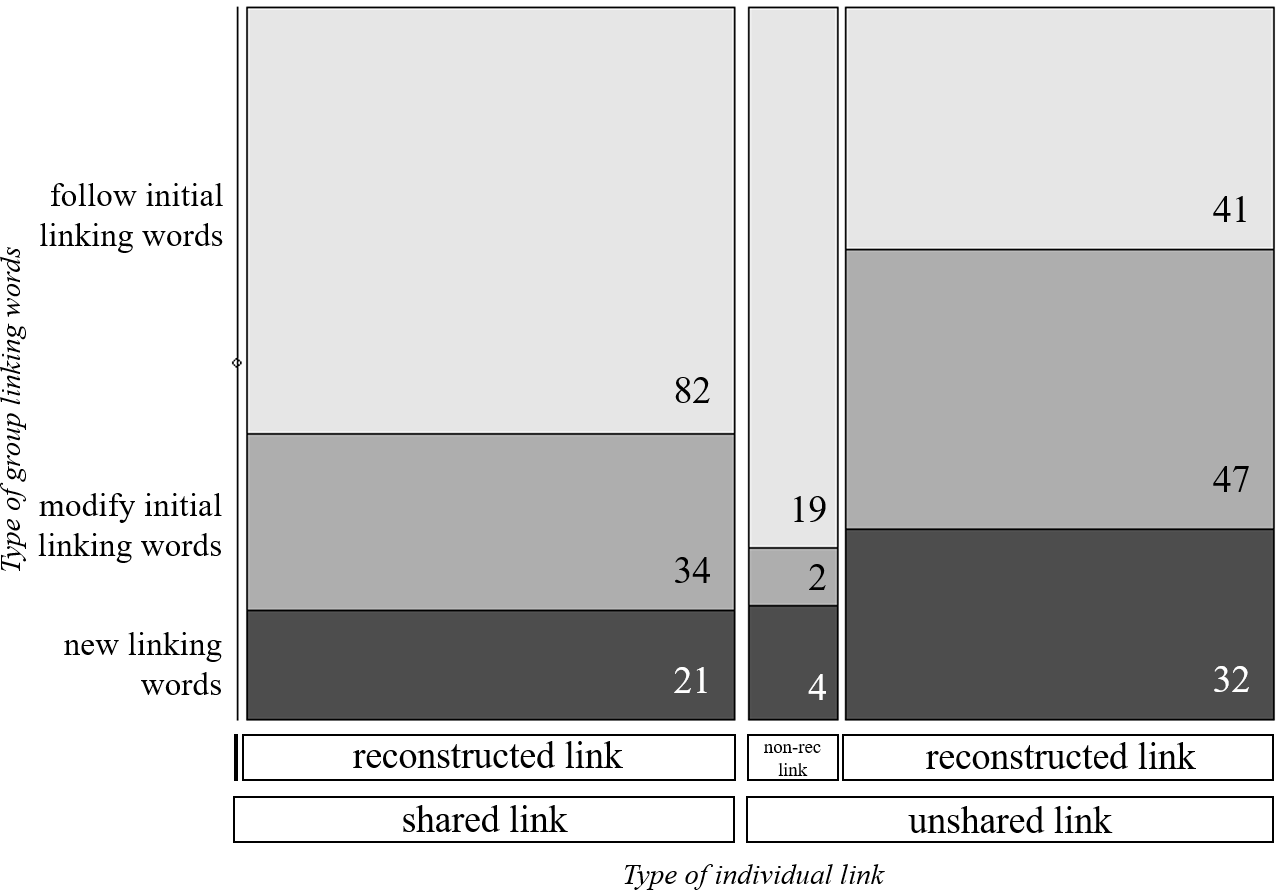
\includegraphics[width=70mm]{/images/a3_group_link_source_1.pdf}
        \end{center}
        \caption{Source of group map components}
        \label{group_link_s1}
    \end{figure}
\end{frame}

\begin{frame}{Results (2): Individual Contributions to Collaborative Products}
    \begin{figure}[tb]
        \begin{center}
            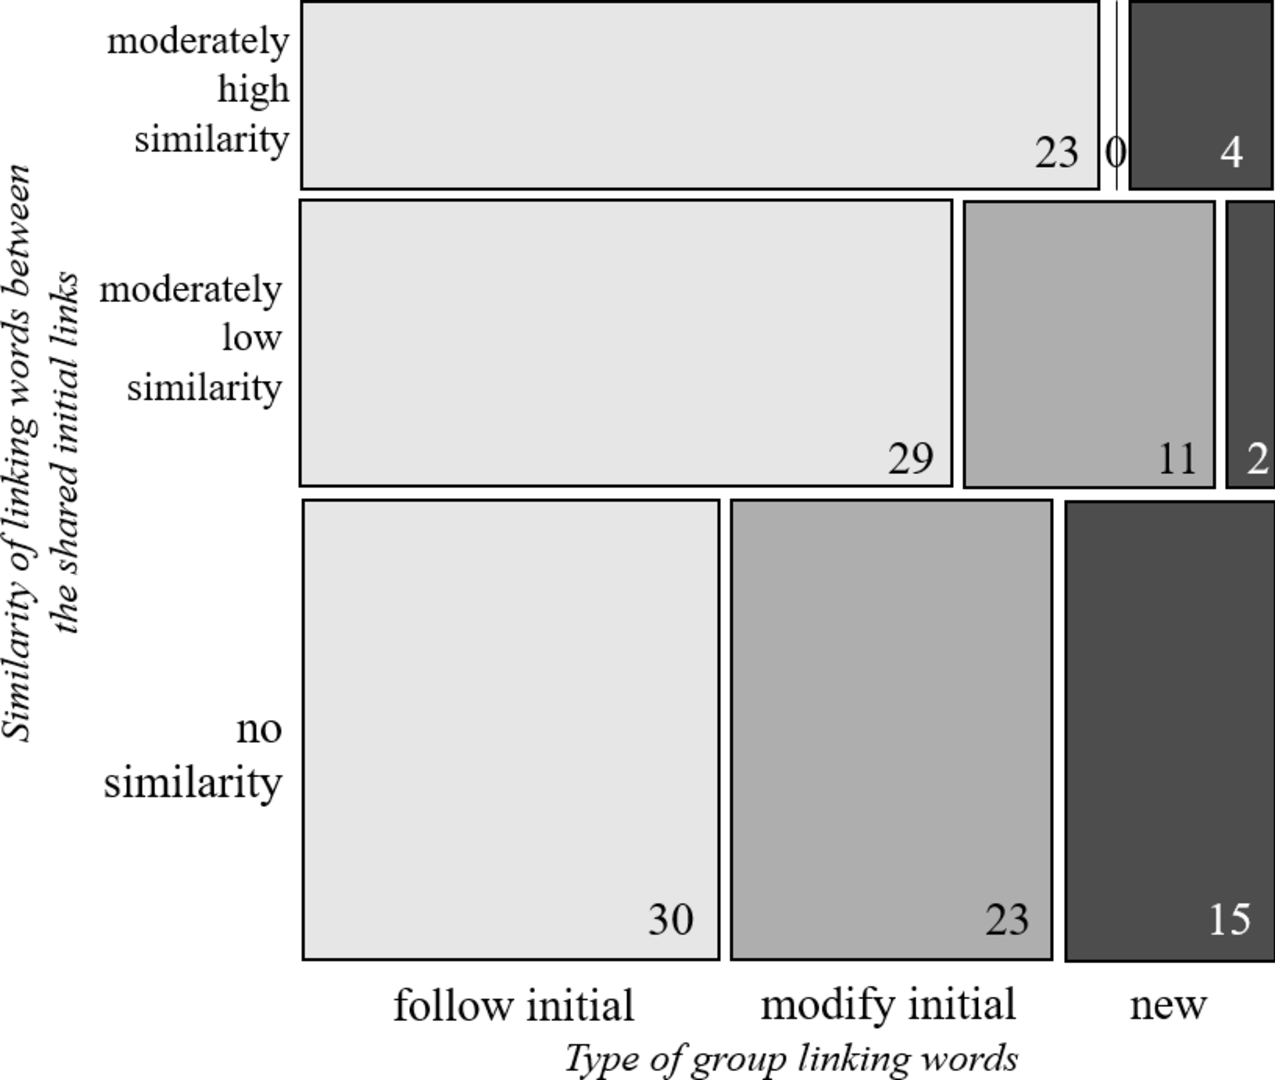
\includegraphics[width=70mm]{/images/a3_group_link_source_2.pdf}
        \end{center}
        \caption{Transfer of individual linking words to group map}
        \label{group_link_s2}
    \end{figure}
\end{frame}


\begin{frame}[allowframebreaks]{Findings}
\begin{enumerate}
    \item does similarity of knowledge or comprehension of partner's rep could be a 
          predictor for collaborative outcome?
          \begin{itemize}
              \item Pearson’s correlation analysis shows that comprehension level and normalized change of products from individual to group level shows a moderately negative correlation, with a significant coefficient, while similarity of prior knowledge reveals a weaker correlation with normalized change. 
              \item The comprehension of the partner’s representation is a stronger predictor to detect the normalized change when compared to the similarity of prior knowledge.
              \item Providing a set of disconnected partner's map components prompted students to reflect their understanding of their partner's representation.
              \item A Wilcoxon signed-rank test indicates that the median of the similarity score between students' second maps and their partners' first maps $(Mdn = .746)$ is significantly higher than the median of the similarity score between students' second and first maps $(Mdn=.6), Z= 224.5, p<0.01$.
              \item When students reconstructed their partners' components,  they were making an effort to understand their partners' maps, rather than to express their own initial maps by using new components.
          \end{itemize}
          
    \item how individual prior knowledge convergence and comprehension 
          levels through reconstruction may potentially influence the final collaborative product.
          \begin{itemize}
            \item The numbers of shared and unshared links in the group solutions are proportionally distributed.
            \item While constructing a group map, the students were tempted to manipulate their first map components rather than creating new links
            \item The students were reflecting on their individual avail-able knowledge to construct the group product.
            \item The results also demonstrate a considerable number of reconstructed unshared links in the group map, which could indicate that the students were able to accept reconstructed elements as parts of group solutions, although they involved different representations. 
            \item Many initial linking words with zero similarity scores from the shared links were modified, which reveals that the students attempted to resolve conflicts regarding different link definitions.  
            \item In contrast, the individual linking words with higher similarity scores were more likely to be included in the group map without any modification.
          \end{itemize}
\end{enumerate}
    
\end{frame}

\begin{frame}{Sample of map transformation}
    \begin{figure}[tb]
        \begin{center}
            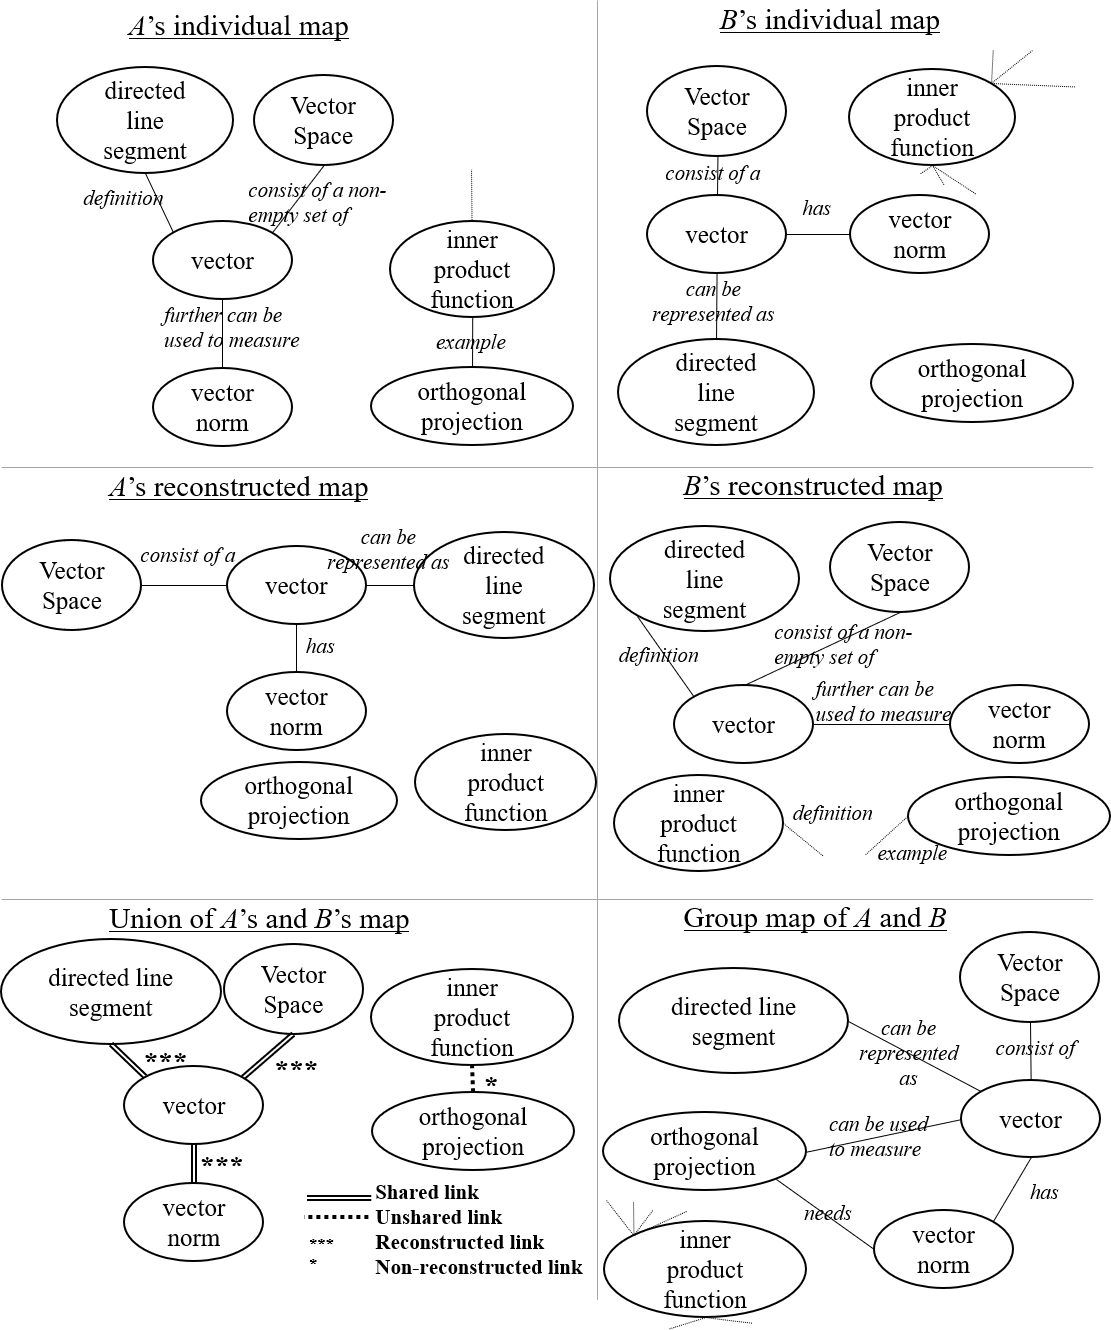
\includegraphics[width=50mm]{images/a3_sample_of_map.pdf}
        \end{center}
        \caption{Sample of individual maps of two students in a group, their reconstructed maps,
            the corresponding union map with the categorization of links, and the 
            newly transformed group map}
        \label{map_sample}
    \end{figure} 
\end{frame}


